% !TEX root = presentation.tex



\begin{frame}[t,fragile]  %Use t argument to align text from the top.  Use fragile argument to include listings in slides
  \frametitle{Getting Started}
  \begin{itemize}
  \item All code and slides are in GIT repo \url{https://github.com/jalving/JuMPTutorial_2018.git}
    \item We will use {\tt Julia} notebooks that will be executed on {\tt JuliaBox}
    \item Access \url{http://juliabox.com}
    \item Click on Sync tab and clone GIT repo \url{https://github.com/jalving/JuMPTutorial_2018.git}
    \item Click on Jupyter tab and access notebooks under JuMPTutorial_2018
    \item Open  {\tt install_packages.ipynb}, click on "Cell" and then on "Run All"
  \end{itemize}
\end{frame}

\begin{frame}
    \frametitle{Optimization Overview}
    \begin{block}{Standard Nonlinear Programming (NLP) Problem}
    \begin{alignat*}{3}
        &\min_x &&f(x)  &&\quad\text{Objective function (e.g., economics)}\\
        &s.t.\ \ &&c(x) = 0\ \  &&\quad\text{Equality constraints (e.g. physical equations)} \\
        & &&g(x) \ge 0 \ \ &&\quad\text{Inequality constraints (e.g. physical limits)}
    \end{alignat*}
    \end{block}
    This tutorial considers PDE-constrained optimization problems, which we will cast as standard NLPs.
    \begin{exampleblock}{Example NLP}
        \vspace{-0.5cm}
        \begin{align*}
            \min_{x_1,x_2} \ \ &x_1^2 + x_2^2\\
            s.t. \ \ &x_1 + x_2 = 5\\
            &e^{x_1} \le 4\\
        \end{align*}
        \vspace{-1.2cm}
    \end{exampleblock}
\end{frame}

\begin{frame}[t]
    \frametitle{Ipopt - Interior Point OPTimizer}
    \begin{footnotesize}
    \begin{itemize}
      \item To solve NLPs we will use the interior-point NLP solver {\tt Ipopt}.
      \item {\tt Ipopt} uses a logarithmic barrier to transform the NLP into an equality-constrained subproblem:
    \end{itemize}
    \end{footnotesize}
    \vspace{-0.5cm}
    \begin{columns}
      \column[T]{0.5\textwidth}
      \begin{figure}[h]
        \centering
        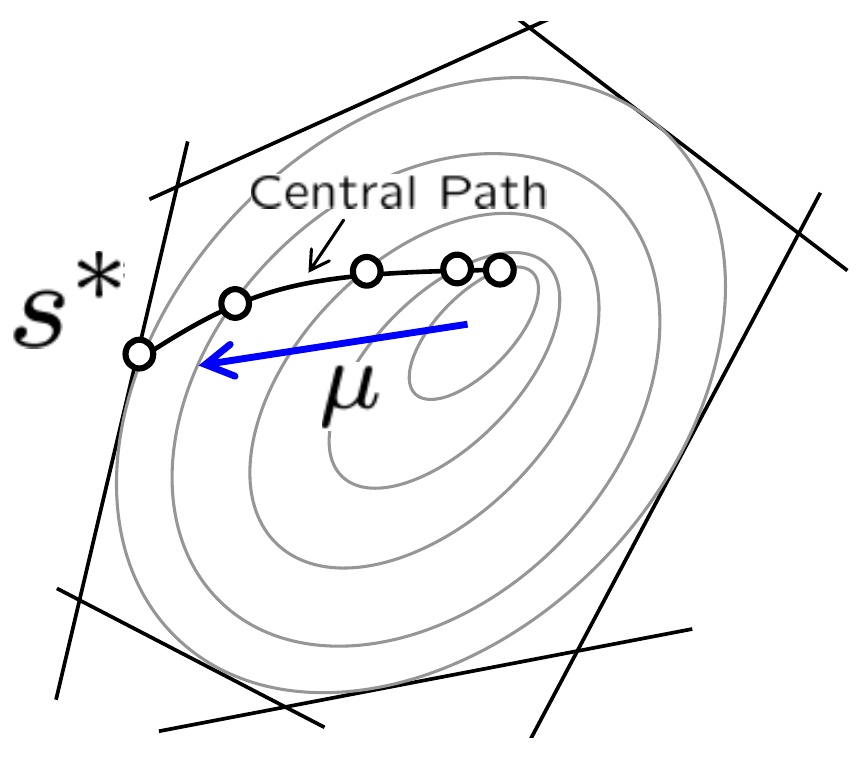
\includegraphics[scale=0.1]{interior_point.png}
      \end{figure}
      \column[T]{0.5\textwidth}
      \begin{footnotesize}
        \scalebox{0.9}{\parbox{.5\linewidth}{        \begin{align*}
         &\min_x \phi^\mu(x) := f(x) - \mu \sum_{j=1}^{m} ln(g_j(x))\\
         &s.t. \; c(x) = 0 \\
        \end{align*}}}
        \end{footnotesize}
      \end{columns}
              \begin{footnotesize}
      \begin{itemize}
      \item The barrier subproblem is solved for decreasing values of $\mu$ to reach a solution of the original NLP. This is done by solving:
      \begin{footnotesize}
  \begin{columns}
     \hspace{0.2in} \column[T]{0.4\textwidth}
              \scalebox{0.9}{\parbox{\linewidth}{        \begin{align*}
            \nabla_{x}\mathcal{L}(x,\lambda)=\nabla_x \phi^\mu(x) +\nabla_x c(x)\lambda&=0\\
           c(x) &= 0 \\
        \end{align*}}}
        \column[T]{0.7\textwidth}
                      \scalebox{0.9}{\parbox{\linewidth}{        \begin{align*}
               \Longrightarrow       \left[\begin{array}{cc}H(x,\lambda)& \nabla_x c(x) \\ \nabla_x c(x)^T\end{array}\right]\left[\begin{array}{c}\Delta x\\ \Delta \lambda \end{array}\right]=-\left[\begin{array}{c}\nabla_x\mathcal{L}(x,\lambda) \\ c(x) \end{array}\right]
       \end{align*}}}
        \end{columns}
        \end{footnotesize}
        \vspace{-0.2in}
      \item Highly efficient sparse linear algebra and globalization strategies enable solution of complex NLPs.
      \item {\tt Ipopt} can solve NLPs with {\em millions} of variables and constraints.
      \end{itemize}
      \end{footnotesize}
\end{frame}

\begin{frame}[t]
    \frametitle{Julia and JuMP}
    \begin{columns}
      \column[T]{0.5\textwidth}
        {\tt Julia}
        \begin{small}
        \begin{itemize}
          \item Language for high-performance scientific computing
          \item Extensive library of tools  for optimization, statistics, plotting, graphs,...
          \item Performance comparable to C
          \item Designed to enable parallelism
        \end{itemize}
        \end{small}
      \column[T]{0.5\textwidth}
        {\tt JuMP}
        \begin{small}
        \begin{itemize}
            \item Algebraic modeling language for optimization written in {\tt Julia}
            \item Syntax close to natural mathematical expressions
            \item Processes problems at speeds comparable to {\tt GAMS} and {\tt AMPL}
            \item Support for open source \& commercial solvers (e.g. {\tt Ipopt}, {\tt Gurobi})
            \item Automatic computation of derivatives
        \end{itemize}
        \end{small}
    \end{columns}
\end{frame}

\begin{frame}[fragile,t]
  \frametitle{Solving Optimization Problems with JuMP}
  Consider our previous NLP example:
  \begin{columns}
    \column{0.1\textwidth}
    \column{0.25\textwidth}
      \begin{align*}
          \min_{x_1,x_2} \ \ &x_1^2 + x_2^2\\
          s.t. \ \ &x_1 + x_2 = 5\\
          &e^{x_1} \le 4\\
      \end{align*}
    \column{1.5\textwidth}
      \lstset{ basicstyle = \scriptsize}
      \begin{lstlisting}
        using JuMP
        using Ipopt
        m = Model()
        @variable(m,x1)
        @variable(m,x2)
        @objective(m,Min,x1^2 + x2^2)
        @constraint(m,x1+x2 == 5)
        @NLconstraint(m,exp(x1) <= 4)
        solve(m)
      \end{lstlisting}
    \vspace{0.0cm}
  \end{columns}
 - {\tt Ipopt} internally solves a sequence of barrier problems of the form:
        \begin{align*}
          \min_{x_1,x_2} \ \ &x_1^2 + x_2^2-\mu \log (4-e^{x_1})\\
          s.t. \ \ &x_1 + x_2 = 5
      \end{align*}
- Example implemented in Julia notebook {\footnotesize {\tt simple_model.ipynb}}
\end{frame}

\begin{frame}[fragile,t]
  \frametitle{Solving Optimization Problems with JuMP}
  {\tt JuMP} also enables compact syntax expressions:
  \begin{columns}
    \column{0.1\textwidth}
    \column{0.25\textwidth}
      \begin{align*}
          \min_{x_1,x_2} \ \ &\sum_{j\in \{1,2\}}x_j^2\\
          s.t. \ \ &\sum_{j\in \{1,2\}}x_j= 5\\
          &e^{x_1} \le 4\\
      \end{align*}
    \column{1.5\textwidth}
      \lstset{ basicstyle = \scriptsize}
      \begin{lstlisting}
        using JuMP
        using Ipopt
        m = Model()
        S = collect(1:2)
        @objective(m,Min,sum(x[j]^2 for j in S))
        @variable(m,x[S])
        @constraint(m,sum(x[j] for j in S) == 5)
        @NLconstraint(m,exp(x[1]) <= 4)
        solve(m)
      \end{lstlisting}
    \vspace{0.5cm}
  \end{columns}
 Example implemented in Julia notebook {\footnotesize{\tt simple_model_set.ipynb}}
\end{frame}

\begin{frame}
    \frametitle{MILP Problems}
    \begin{block}{Standard Mixed Integer Linear Programming Problem}
    \end{block}

\end{frame}
